\chapter{Numerical Experiments}
In this chapter, we will solve the eigenvalue problem, Eq.(\ref{eq:eigenvalue-problem}), with different discretizations. There will be three major categories of methods used. Finite difference (FD) method, finite element (FE) method and discrete variable representation (DVR) method.

The finite difference method will be used together with equally spaced nodes. The finite element method will be used with three different basis functions: tent function, B-spline and sine. Different basis function results in different discretization. Finally, sine DVR and sinc DVR will also be used to solve the eigenvalue problem.

The parameters of different discretizations are listed below
\begin{table} [H]
	\begin{tabular}{|c|c|c|c|c|c|c|}
		\hline
		& FD & FE\_TENT & FE\_BSPLINE & FE\_SINE & DVR\_SINE & DVR\_SINC \\
		\hline
		N & 201 &  &  &  &  &  \\
		\hline
		NUM\_BASIS &  & 15 & 21 & 50 & 31 & 39 \\
		\hline
	\end{tabular}
	\label{table:parameters}
\end{table}

\section{Constant Velocity}
Because the existence of exact solution to problems Eq.(\ref{eq:constant_v_problem_dirichlet}) and Eq.(\ref{eq:constant_v_problem_openright}). The case with constant velocity profile is used as a sanity check. It allows us to verify the correctness of each method's implementation. This also serves as a reference to the accuracy spectral methods can achieve.

From Fig.(\ref{fig:constant_v}), we see that the flow in magnetic nozzle with subsonic and supersonic velocity profile are both stable. The accuracy of spectral method is high, the imaginary part of eigenvalues are about $10^{-13}$.

\begin{figure}[H]
	\centering
	\begin{subfigure}{0.5\textwidth}
		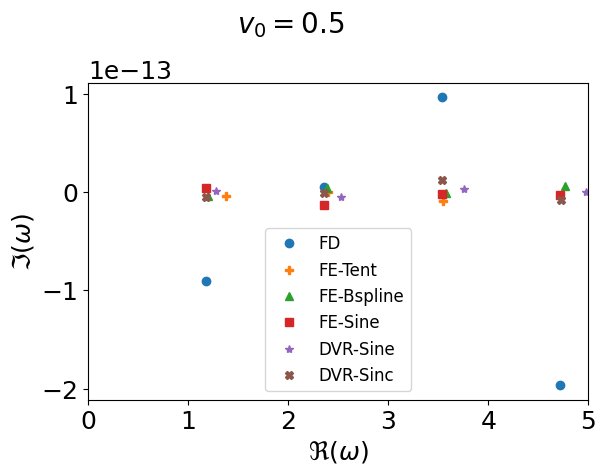
\includegraphics[width=\linewidth]{img/numerical_experiments/constant_v_v0=0.5}
		\caption{Subsonic}
	\end{subfigure}%
	\begin{subfigure}{0.5\textwidth}
		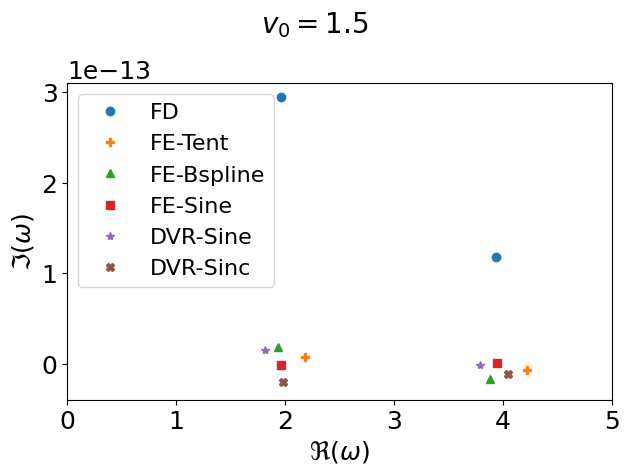
\includegraphics[width=\linewidth]{img/numerical_experiments/constant_v_v0=1.5}
		\caption{Supersonic}
	\end{subfigure}
	\caption{In subsonic case, all methods produces stable modes. In supersonic case, all modes are stable after filtering the spurious modes.}
	\label{fig:constant_v}
\end{figure}


\section{Subsonic Case}
\subsection{Fixed Ends}
With Dirichlet boundary condition, $\tilde{v}(\pm 1) =0$. The flow in magnetic nozzle with subsonic velocity profile is stable. Fig.\ref{fig:subsonic_v} shows the first few eigenvalues obtained by different discretizations, they all produced similar results.
\begin{figure} [H]
	\centering
	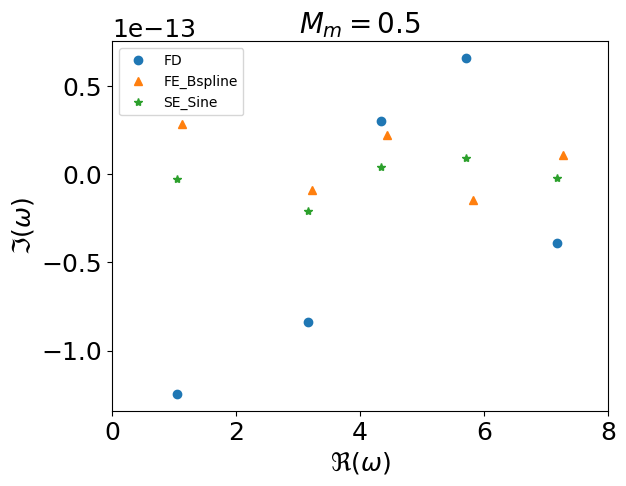
\includegraphics[width=0.7\linewidth]{img/numerical_experiments/subsonic_v}
	\caption{The flow is stable.}
	\label{fig:subsonic_v}
\end{figure}

\subsection{Open Right End}


\section{Supersonic Case}
\subsection{Fixed Ends}
When the velocity profile is supersonic, spurious modes appeared as predicted in Chap.\ref{chap:theoretical_analysis}. Using the convergence test, we successfully eliminates all spurious modes. Fig.(\ref{fig:supersonic_v}) shows the first few filtered eigenvalues. As we can see the flow is stable.
\begin{figure} [H]
	\centering
	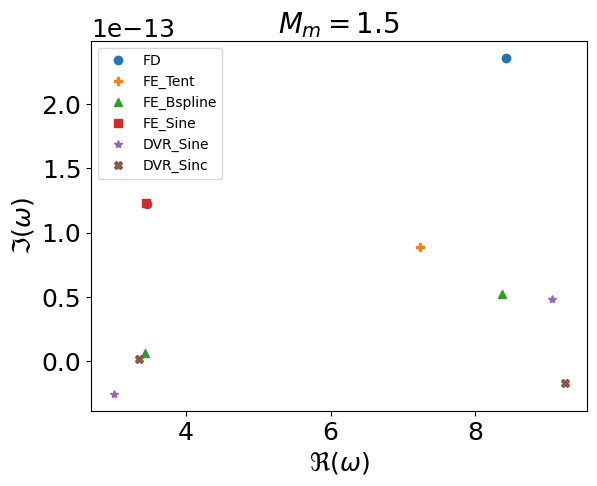
\includegraphics[width=0.7\linewidth]{img/numerical_experiments/supersonic_v}
	\caption{First few filtered eigenvalues are shown. The spurious modes are filtered by convergence test.}
	\label{fig:supersonic_v}
\end{figure}

\subsection{Open Right Ends}


\section{Accelerating Case}
In this case, the flow starts from subsonic speed and accelerates to supersonic case, the velocity is exactly at sonic point $M_m=1$ at the center of the magnetic nozzle as shown in Fig.(\ref{fig:velocity_profiles})
\subsection{Fixed Ends}
With Dirichlet boundary condition, spectral method with different discretizations gave negative eigenvalues. This indicates that the perturbation $\tilde{v}$ is damped oscillation, its amplitude will be decrease to zero exponentially in time, $\tilde{v} \sim \exp(\Im(\omega)t)$. Hence, the flow in magnetic nozzle is stable.
\begin{figure} [H]
	\centering
	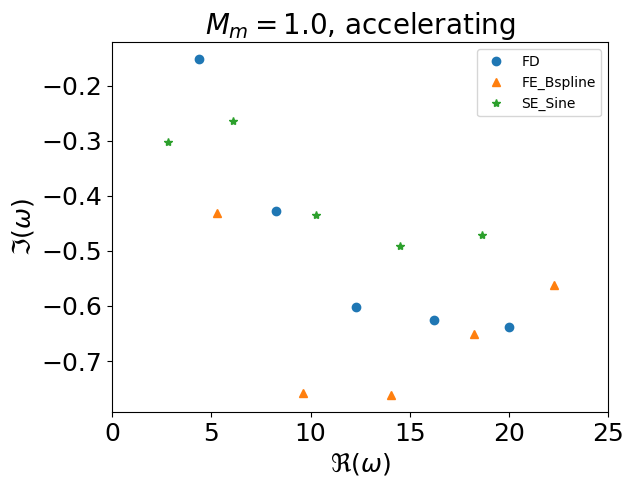
\includegraphics[width=0.7\linewidth]{img/numerical_experiments/accelerating_v}
	\caption{The filtered eigenvalues are negative. This indicates that the perturbation $\tilde{v}$ is a damped oscillation, their amplitude will decrease to zero as time elapse.}
	\label{fig:accelerating_v}
\end{figure}

\subsection{Open Right Ends}


\section{Decelerating Case}
\subsection{Fixed Ends}
Let $v_a(z)$ denotes the accelerating velocity profile, and $v_d(z)$ the decelerating velocity profile. Then we know $v_a(-z) = v_d(z)$.

The eigenvalue problem with accelerating profile is given by
\[
	\hspace{-0.5in}
	\omega^2 \tilde{v} 
	+ 2i\omega\left(v_a\pdv{}{z} + \pdv{v_a}{z}\right) \tilde{v} 
	+ \left[ (1-v_a^2)\pdv[2]{}{z} 
	-\left(3v_a + \frac{1}{v_a}\right)\pdv{v_a}{z}\pdv{}{z} 
	- \left(1-\frac{1}{v_a^2}\right)\left(\pdv{v_a}{z}\right)^2 
	- \left(v_a+\frac{1}{v_a}\right)\pdv[2]{v_a}{z} \right]\tilde{v}
	= 0
\]
Let $z\mapsto -z$, the eigenvalue problem becomes
\[
	\hspace{-1.5in}
	\omega^2 \tilde{v} 
	+ 2i\omega\left(v_d\pdv{}{(-z)} + \pdv{v_d}{(-z)}\right) \tilde{v} 
	+ \left[ (1-v_d^2)\pdv[2]{}{(-z)} 
	-\left(3v_d + \frac{1}{v_d}\right)\pdv{v_d}{(-z)}\pdv{}{(-z)} 
	- \left(1-\frac{1}{v_d^2}\right)\left(\pdv{v_d}{(-z)}\right)^2 
	- \left(v_d+\frac{1}{v_d}\right)\pdv[2]{v_d}{(-z)} \right]\tilde{v}
	= 0
\]
Hence, we have
\[
\hspace{-0.5in}
\omega^2 \tilde{v} 
- 2i\omega\left(v_d\pdv{}{z} + \pdv{v_d}{z}\right) \tilde{v} 
+ \left[ (1-v_d^2)\pdv[2]{}{z} 
-\left(3v_d + \frac{1}{v_d}\right)\pdv{v_d}{z}\pdv{}{z} 
- \left(1-\frac{1}{v_d^2}\right)\left(\pdv{v_d}{z}\right)^2 
- \left(v_d+\frac{1}{v_d}\right)\pdv[2]{v_d}{z} \right]\tilde{v}
= 0
\]

We see that the flow with decelerating profile is a different physical process than the that with accelerating profile.

\begin{figure} [H]
	\centering
	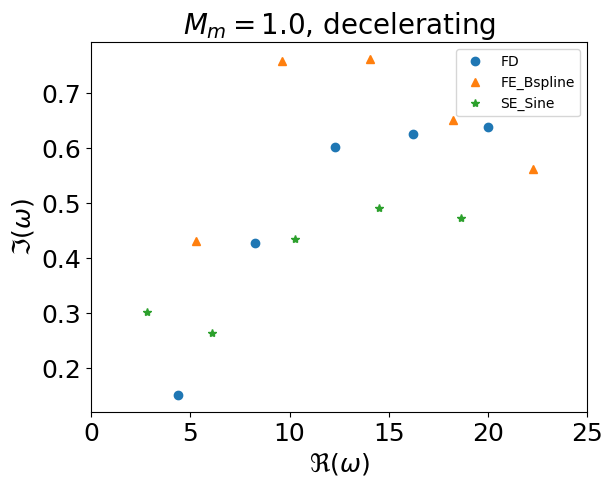
\includegraphics[width=0.7\linewidth]{img/numerical_experiments/decelerating_v}
	\caption{Unstable}
	\label{fig:decelerating_v}
\end{figure}

\subsection{Open Right Ends}
